%\documentclass{article}
%\usepackage{ijcai13}
%\usepackage{times}
%\usepackage{latexsym} 

\documentclass[letterpaper]{article}
\usepackage{aaai}
\usepackage{times}
\usepackage{helvet}
\usepackage{courier}
\usepackage{algorithm2e}
\frenchspacing

\usepackage{graphicx}

\title{Social Computing Article\thanks{This title is temporary}}

\begin{document}

\maketitle

\begin{abstract}
  Abstract
\end{abstract}

\section{Introduction}

For years multi-agent systems have been used to research cooperation as a tool for problem-solving. Recently, however, there has been an increasing interest in the study of human beings as problem-solving agents. Several experiments have been conducted in which subjects are connected in a network with the goal of collectively solving a specific problem, and those have helped shed some light on the way humans interact to solve problems. However, although those studies can provide us with observations and hypotheses, there is still a difficulty in finding ways to explain the observed behaviour. In this paper, we use a multi-agent based simulation to complement the study of human computation, as a way of explaining the strategies used by humans and understanding their consequences in a cooperative environment. The control that simulations provide us over the behaviour of the agents allows us to better understand possible reasons for the ones displayed by humans.

Human beings are known to be able to easily perform tasks which are still generally difficult for computers, such as natural language processing and image recognition. However, it would be useful to be able to apply human social computation to more straightforward computer problems with precise definitions and algorithms, but which are still computationally intensive. The different sets of abilities between computers and humans suggest that the latter might provide a new approach to those problems that might be more effective than current techniques employed by computers. That notion has been successfully applied, for example, in one of the most significant problems in the field of bioinformatics: protein structure prediction (PSP). A software that presents the problem to humans as an online computer game, called \emph{Foldit} \cite{cooper:foldit}, has produced significant results in the research of PSP, which is usually approached as an optimization problem requiring extensive computational power. Those results have been attributed to human visual problem-solving and decision-making abilities, as well as social collaboration \cite{cooper:foldit}. However, we still don't know the limits of human abilities in problem-solving and how they compare to more traditional techniques. To take full advantage of human problem-solving strategies, we must learn their limitations. In order to obtain that knowledge, our system simulates human behaviour according to findings of social computation experiments.

\section{Background}

Social computation is a relatively new area of research with a diversified, interdisciplinary root that mixes social sciences, artificial intelligence, game theory and network science, among others. Only recently studies on the potential of human social networks for solving problems are gaining some popularity. Those have provided insights into, among other things, the impact of network structure in the collaboration process and the factors that lead neighbours' proposed solutions to be copied by individuals.

The origin of human computation as we know it today can be traced back to the work of \cite{vonahm:gwap}, which identified the possibility of using entertainment as an incentive to participation of human subjects, applying it in games in which the participants are actually performing a computation. That is an idea that also appears in the Foldit game.

The series of experiments summarized in \cite{kearns:experim} are among the first to try to take advantage of the collective's problem-solving abilities to solve classical computer problems. The experiments are mostly based on the concept of coordination: subjects have individual incentives that are expected to drive them to cooperate with one another and lead them toward the collective goal.

Other initiatives have appeared, such as the ones by \cite{farenzena:collabem} and \cite{mason:collablearnet}, which take a different approach by having subjects trying to solve the collective problem individually, with the possibility of exchanging solutions between neighbours. Those have resulted in interesting conclusions on human behaviour when the possibility of copying peers makes itself present. It's in those models of experiments that we will focus in this work.

The experiments conducted by \cite{farenzena:collabem} had human beings trying to solve constraint satisfaction problems, namely Boolean Satisfiability (SAT) and the popular \emph{Sudoku} game, with individuals connected through the network being able to exchange partial solutions of the problem in question. There were two main patterns of behaviour observed in this study in regard to copying neighbours' solutions:

\begin{itemize}
	\item Humans might not evaluate the solutions proposed by their peers, instead choosing the most readily available one. On the other hand, \cite{mason:collablearnet} suggest that their subjects did evaluate the available solutions, although an in-depth analysis of that wasn't provided.
	\item There is a higher probability of individuals copying peers' solutions when those are shared by several neighbours. That behaviour is referred to by the authors as \emph{conformism}. A similar behaviour was observed by \cite{mason:collablearnet}, even though the experiments used a different problem.
\end{itemize}

\cite{mason:collablearnet} also provided important insights to human cooperation. However, since our basis is the work of \cite{farenzena:collabem} we will use the former's results only as secondary support.

\section{Contribution}

We have built a multi-agent system that simulates the experiments of \cite{farenzena:collabem}, using the model of human behaviour proposed by them. We adapted that behaviour into a set of rules which we modeled in the \emph{Memetic Network} model proposed by \cite{lamb:memenet}. For simplicity, we limited our experiments to the Sudoku problem. Our goal is verifying whether the strategies employed by humans are competitive with other heuristics. After identifying the points in which those are lacking, we will then propose methods to increase the efficiency of human problem-solving networks.

\section{System Overview}

We developed a system in which the environment of the {\em Sudoku} problem-solving social network presented in~\cite{farenzena:collabem} could be modelled through autonomous agent networks and analysed through a series of experiments. We conceived a novel method for agent-based social problem solving witch draws inspiration from the optimization technique of {\em Memetic Networks}~\cite{lamb:memenet}.

\section{A Novel Method for Agent-based Social Problem Solving}

A number of multi-agent methodologies that employ information flow through agents have been studied before. For instance, the {\em Memetic Networks} model proposed by~\cite{lamb:memenet} draws inspiration from the phenomenon of {\em Cultural Evolution} discussed by Dawkins in~\cite{dawkins:selfishgene} and has a network of agents sharing, copying and incrementing units of information in a similar way that nature, according to Dawkins, deals with {\em Memes}~\cite{dawkins:selfishgene}. Nevertheless, some aspects of social behaviour of great significance to social computing cannot be properly analysed through this methodologies. One example is the conformist behaviour studied in~\cite{cefferson:conformists} and~\cite{farenzena:collabem}. The proper study of these aspects demands a novel method for agent-based collaborative problem solving.

We propose a method for solving computational problems by the means of a network of agents with social behaviour. Our algorithm is composed of an ordered set of $N$ agents, each encoding a partial solution to the problem, and a binary $N \times N$ matrix representing possible connections between agents. Additionally, our algorithm is composed of two stages, namely the {\em Social Stage} and the {\em Cognitive Stage}. 

\begin{itemize}
\item
Social Stage: In the {\em Social Stage}, messages are passed from agent to agent through the network connections. Agents are thus presented with a multiplicity of messages. There is a particular probability associated with the behaviour of agents choosing to copy one of these solutions in contrast to keeping their current solutions. We call this probability the {\em Copy Rate}. When an agent chooses to copy, he or she is then supposed to select for copying only one of his or her received messages. This is done by the means of a particular message-selecting metric.

\item
Cognitive Stage: In the {\em Cognitive Stage}, agents are supposed to add local changes to the messages copied in the previous stage. This is done by the means of a heuristic or an exact method.
\end{itemize}

\begin{algorithm}
 \SetAlgoLined
 Initialize N agents, each encoding a partial solution to the problem\;
 \While{termination condition not met}
 {
 	\For{i = 1 to N}
 	{
 		\For{j = 1 to N}
 		{
 			\If{j is connected to i}
 			{
 				A = $i_{th}$ agent\;
 				A.messages.add(j.solution)\;
 			}
 		}
 	}
 	\For{i = 1 to N} 
 	{
 		\CommentSty{ //Social Stage }\;
 		A = $i_{th}$ agent\;
 		selectedMessage = select(A.messages)\;
 		
 		\If{random(0,1) $<$ copyRate}
 		{
 			A.solution = selectedMessage\;
 		}
 	}
 	\For{i = 1 to N}
 	{
 		\CommentSty{ //Cognitive Stage }\;
 		A = $i_{th}$ agent\;
 		A.solution = addLocalChanges(A.solution)\;
 	}
 }
 \caption{No name yet}
\end{algorithm}

\section{Performance Tests}

In order to validate the algorithm as a social problem solving technique, we have modelled the collaborative {\em Sudoku} solving environment studied in~\cite{farenzena:collabem} through it and tested it over a set of {\em Sudoku} instances.

\subsection{Social Stage}

The experiments conducted by~\cite{farenzena:collabem} point out a series of observations about the dynamics of cooperation in problem solving with human beings. For instance, the authors analysis has shown that human subjects are more likely to engage in the behaviour of copying the most readily available solutions on the graphic interface than in that of copying the most complete solutions. In order to analyse and compare this two behaviours, he have modelled each one of them as a message-selecting metric for the {\em Social Stage}.

\subsubsection{{\em Pick Most Filled} metric}

This metric employs the intuitive strategy of selecting the most complete message for copying. In the specific case of {\em Sudoku} solving, this metric selects the most filled {\em Sudoku} partial solution. Put in other words, it selects the {\em Sudoku} partial solution with the lesser number of blank cells.

\subsubsection{{\em Pick Among First} metric}

We know that, in some settings of collaborative problem-solving, human subjects are likely to copy the first (from left to right) solutions on the graphic interface~\cite{farenzena:collabem}. The authors have provided us with a mathematical model of this behaviour, stated as $\langle X(k)\rangle = (1-p)^{k-1}p$, where the parameter $p$ is fixed as $p = 0.5479$ and $\langle X(k)\rangle$ denotes the probability of an agent copying the $k_{th}$ neighbour solution.

We inserted this behaviour into our model by firstly generating a random ordering of neighbours for each agent in order to compose a simulated graphic interface. As a result, each agent visualizes some neighbours before or after others. Secondly, we translated the above mathematical model into an message-selecting metric in which the solution selected by an agent is the $k_{th}$ with probability $\langle X(k)\rangle$.

\subsection{Cognitive Stage}

{\em Sudoku} solving techniques are abundant in {\em Sudoku} strategy literature.Davis ~\cite{davis:mathsudoku} discusses a collection of these techniques, of which the {\em Naked Singles} rule, the {\em Hidden Singles} rule and the {\em Naked Twins} rule are some examples. These techniques intend to, given a partial {\em Sudoku} solution, generate a set of {\em movements} which can be used to mark cells of this {\em Sudoku} puzzle. We implemented $4$ of these rules, modelling each one of them as a function that maps a {\em Sudoku} partial solution to a set of {\em movements}. These functions can be used in the {\em Cognitive Stage} to add local changes to the {\em Sudoku} message received in the {\em Social Stage}.

\subsubsection{Only Choice}

This technique marks a {\em Sudoku} cell with a value only if this cell is the last blank cell on its row, column or $3 \times 3$ block.

\subsubsection{Naked Singles}

This rule marks a {\em Sudoku} cell with value $v$ only if $v$ is the single possible value to mark that cell. The other values must have been eliminated through a process of verifying that they are all present in the span encompassing the cell's row, column and $3 \times 3$ block.

\subsubsection{Hidden Singles}

This rule is similar to the {\em naked singles} rule. It is able to mark cells with more than one candidate value by looking for cells that are the only ones in their row, column or $3 \times 3$ block that can hold a particular value.

\subsubsection{Two out of Three}

This rule applies to groups of three contiguous $3 \times 3$ blocks. It aims to find a value $v$ such that $v$ is present in two of the three $3 \times 3$ blocks encompassed by the group, but missing on the third. It proceeds by enumerating all the candidate cells - namely the empty cells - on this block, and then, by eliminating from this set all the cells that are encompassed by the rows or columns in which $v$ is placed on the other two blocks. If the resulting set has cardinality $1$, the rule has successfully found a cell to mark.

\subsubsection{Naked Twins}

\subsection{Copying Solutions}

In a study conducted by~\cite{farenzena:collabem}, subjects were invited to solve {\em Sudoku} puzzles and share them with other subjects with whom they were connected through a network topology. At any time, a player could copy solutions from one of his or her neighbours. The authors' analysis has shown that there is a different copy frequency associated with each topology. For instance, the scale free topology with $\gamma = 1.65$ resulted in a copy frequency of $87 \%$, while the fully connected topology resulted in a copy frequency of $42 \%$.

We incorporated this copying frequency into our modelling, recreating the scenario of the experiments conducted by~\cite{farenzena:collabem} by setting this parameter accordingly to the topologies we used.

\subsection{Conformist Behaviour}

We introduce in our modelling the {\em conformist} behaviour proposed by~\cite{cefferson:conformists} and further studied by~\cite{farenzena:collabem}, which states that agents are likely to copy a particular solution with probability $1$ when surrounded by neighbours that share this solution. 

Our approach was to establish a {\em treshold} determining a minimum necessary quantity $N$ of neighbours sharing a particular solution. In our modelling, all agents with $N$ or more neighbours having a solution $s$ in common are programmed to copy solution $s$ from them.

\subsection{Guessing and Backtracking}

We have consistent evidence that trial-and-error is a part of the {\em Sudoku} solving experience. The need for trial-and-error in {\em Sudoku} puzzles is not a falsifiable conclusion, but a mathematical fact~\cite{davis:mathsudoku}. Some puzzles are only solvable by the means of a backtracking procedure (see Figure 1).

\begin{figure}
\centering
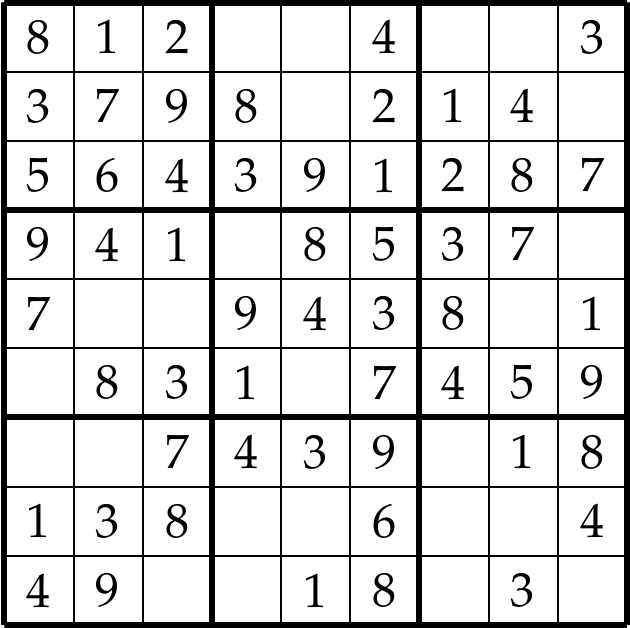
\includegraphics[scale=0.30]{trial_and_error_sudoku}
\caption{A {\em Sudoku} puzzle solvable only by trial-and-error}
\label{fig:trial_and_error_sudoku}
\end{figure}

In our modelling, we associate each agent with a numerical parameter determining the probability of this agent to guess when incapable of applying a typical {\em Sudoku} solving strategy.

Automatic {\em Sudoku} solvers employing a backtracking algorithm are easily programmed and very time-efficient. On the other hand, the space complexity of these algorithms is a barrier to most human solvers, who need to write down tons of observations in order to employ a backtracking strategy. With this in mind, we propose in our modelling two different kinds of backtracking, intended to be more similar to the way human beings employ error correction in {\em Sudoku} solving in a collaborative environment such as the one analysed in~\cite{farenzena:collabem}.

\begin{itemize}

\item
Local Backtracking: When faced with one or more conflicts in its own solution, an agent simply erases the conflicting cells.
\item
Social Backtracking: When faced with one or more conflicts in its own solution, an agent copies a solution from one of its neighbours. In our modelling, this is done by raising the copy rate of this particular agent to $1$.

\end{itemize}


\section{Results}

Results

\section{Conclusions}

Conclusions

\section{Acknowledgements}

We are grateful to Diego Noble and Cristiano *{\em qual sobrenome?}* for their advice, contribution and proofreading. Research partly supported by CPNPq and CAPES, Brazil.

%% The file named.bst is a bibliography style file for BibTeX 0.99c
\bibliographystyle{named}
\bibliography{Article}

\end{document}

